\chapter{関連研究}

\section{行動情報から信念と欲求を推定する研究}
\par
行動情報から信念と欲求を推定する研究として,人間の心的状態理論Theory of Mind (ToM) \cite{子安増生1997心の理論}をベイズ推定を用いてモデル化し,散策行動から信念と欲求を推定するBayesian Theory of Mind (BToM) \cite{baker2011bayesian}が存在する.BToMは,環境の状態や人間の信念と欲求を部分的に観測可能なマルコフ決定過程\cite{alma9926438829904034}として表し,環境における人間の意思決定をベイズ推定に適用することで,環境中で人間が観測できていない部分についての信念と欲求を推定する.図\ref{fig:btom}に,BToMにおけるベイズ推定を表現するベイジアンネットワーク\cite{alma9926301926204034}を示す.$s_t$および$a_t$は観測値,$o_t$,$b_t$および$d$は確率変数として扱う.
\begin{figure}[htbp]
  \begin{center}
    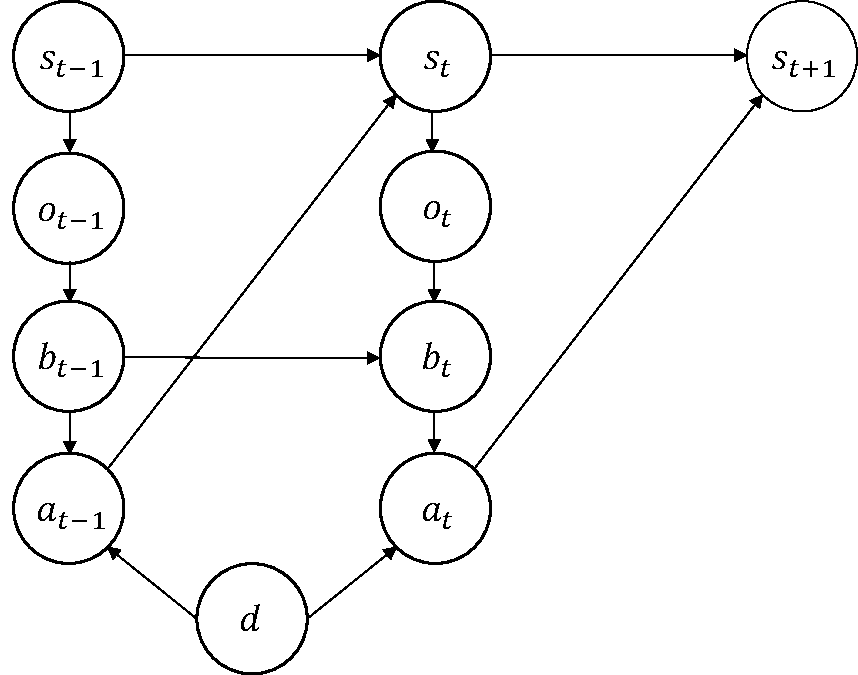
\includegraphics[scale=0.7]{./btom.pdf}
    \caption{BToMにおけるベイズ推定を表現するベイジアンネットワーク}
    \label{fig:btom}
  \end{center}
\end{figure}
BToMにおけるベイズ推定では,時刻$t$における環境の状態$s_{t}$を基に人間の観測状況$o_{t}$が決定される.また,観測状況$o_{t}$を基に人間の信念$b_{t}$が決まり,信念$b_{t}$と欲求$d$から人間の散策行動$a_{t}$が決まる.散策行動$a_{t}$が起こることにより,環境の状態は$s_{t+1}$に変化し,人間の観測状況,信念および散策行動が再び決定される.BToMでは,時刻$1$から時刻$t$までの環境の状態遷移$s_{1:t}$と時刻$1$から時刻$t-1$までの人間の散策行動履歴$a_{1:t-1}$から計算される信念$b_t$と欲求$d$の確率$P(b_t,d|s_{1:t},a_{1:t-1})$を解くことを目的としている.ベイズの定理\cite{ベイズ}と図\ref{fig:btom}における変数間の独立性\cite{ベイズ}より,式(\ref{btom})が成り立つ.
\begin{equation}
  \begin{split}
  \label{btom}
  P(b_t,d|s_{1:t},a_{1:t-1}) &\propto P(b_t,d,s_{1:t},a_{1:t-1})\\
  &= \sum_{b_{t-1},o_t}P(b_t,d,s_{1:t},a_{1:t-1},b_{t-1},o_t)\\
  &= \sum_{b_{t-1},o_t}P(b_t|d,s_{1:t},a_{1:t-1},b_{t-1},o_t)\cdot P(d,s_{1:t},a_{1:t-1},b_{t-1},o_t)\\
  &= \sum_{b_{t-1},o_t}P(b_t|b_{t-1},o_t)\cdot P(o_t|d,s_{1:t},a_{1:t-1},b_{t-1})\cdot P(d,s_{1:t},a_{1:t-1},b_{t-1})\\
  &= \sum_{b_{t-1},o_t}P(b_t|b_{t-1},o_t)\cdot P(o_t|s_t)\cdot P(s_t|s_{t-1},a_{t-1})\\
  &\hspace{3cm} \cdot P(a_{t-1}|b_{t-1},d)\cdot P(b_{t-1},d,s_{1:t-1},a_{1:t-2})\\
  &\propto \sum_{b_{t-1},o_t}P(b_t|b_{t-1},o_t)\cdot P(o_t|s_t)\cdot P(s_t|s_{t-1},a_{t-1})\\
  &\hspace{3cm} \cdot P(a_{t-1}|b_{t-1},d)\cdot P(b_{t-1},d|s_{1:t-1},a_{1:t-2})\\
  \end{split}
\end{equation}
ここで,$P(b_t|b_{t-1},o_t)$は人間の観測$o_t$によって信念$b_t$が更新される確率,$P(o_t|s_t)$は環境の状態$s_t$において人間が観測状況$o_t$を得る確率,$P(s_t|s_{t-1},a_{t-1})$は環境の状態$s_{t-1}$において,人間が散策行動$a_{t-1}$を起こした時に環境の状態が$s_t$になる確率,$P(a_{t-1}|b_{t-1},d)$は人間が信念$b_{t-1}$,欲求$d$を持つ時に散策行動$a_{t-1}$を起こす確率,$P(b_{t-1},d|s_{1:t-1},a_{1:t-2})$は時刻$t-1$におけるBToMの出力である.式(\ref{btom})より,$P(b_t,d|s_{1:t},a_{1:t-1})$は初期値$P(b_1,d|s_1,a_0)$を決めて順次更新する計算により求めることができる.
% また,$P(b_t,d|s_{1:t},a_{1:t-1})$は$P(b_t|b_{t-1},o_t)$,$P(o_t|s_t)$,$P(s_t|s_{t-1},a_{t-1})$および$P(a_{t-1}|b_{t-1},d)$の乗算として表すことができる.


\par
自動車の運転行動から信念や意図を推定する研究 \cite{darwish2020learning}も存在する.自動車の運転では,運転者の信念や意図によりスピードや前方車との車間距離が異なる.また,天候や時間によって運転者が選択する行動は変化する.運転者がどのような行動を起こすことを意図しているかを推定するために,交通状況を部分的に観測可能なマルコフ決定過程として表し,運転者の信念や意図をBToMを用いてモデル化している.その結果,自動運転において運転者の信念や意図に沿った動作の実現を手助けする.

\par
また,作業用ロボットが人間の労働における動作から欲求を推定研究 \cite{inbook}も存在する.人間の作業員のアシスタントとして,人間の欲求を推定することができるロボットを導入することで,効率的かつ安全な作業を行うことを目的としている.この研究における欲求推定においては,人間の欲求の移り変わりも考慮している.

\section{言語情報から信念や欲求を推定する研究}
\par
言語情報から信念と欲求を推定する研究として,人間の発話文から信念や欲求,意図を推定する研究 \cite{高橋拓誠2015bdi}がある.対話相手の意図を考慮した対話を行う対話システムの実現のために,人間の発話文から信念や欲求,意図が推定される.この研究では,Beliefモジュール,Desireモジュール,Intentionモジュールから構成されるモデルを用いて意図を推定する.最初に,Beliefモジュールは発話から事象を抽出し,信念として捉える.Desireモジュールは,Beliefモジュールにおいて捉えられた信念を基に欲求の候補を複数生成する.また,生成された欲求の候補に対し,情緒生起手法 \cite{2002}を適用し,それぞれの尤度を算出し,最も尤度が高いものを欲求とする.Intentionモジュールは,Desireモジュールにおいて選択された欲求を基に意図推定を行う.

\par
検索精度向上のために,言語情報と信念や欲求,意図の関係を適用する研究 \cite{10.1007/978-3-642-02481-8_4}では,ユーザの信念や欲求,意図を考慮し,それを検索に反映することで,よりユーザが欲する情報を提供することに取り組んでいる.

\par
機械翻訳の改善に向けてユーザの信念を活用する研究\cite{farwell1997user}では,ユーザが持つ信念により翻訳の粒度や表現を変えることでユーザの翻訳理解度が向上するという仮説の下,ユーザが入力した文章から信念を推定し,それを基に翻訳の粒度や表現を変え,ユーザが理解しやすい翻訳を提供することに取り組んでいる.

\section{SCAIN}
対話において相手の信念と欲求を推定するためには,対話の文脈と信念と欲求の推定の相互依存性を解決することが必要である.対話において,文脈が相手の信念と欲求の推定に影響を与えたり,相手の信念と欲求により文脈が変わることがある.対話における文脈と単語の解釈の相互依存性を逐次的に解決する研究として,SCAIN \cite{takimoto2020slaminspired}が存在する.対話において,文脈により単語の解釈が変わったり,単語の解釈によって文脈が変わることがあり,対話の文脈と単語の解釈には相互依存性があるといえる.SCAINでは,対話履歴を対話の文脈として捉え,対話の文脈の推定と単語の解釈を並行して行うことで,文脈と単語の解釈の相互依存性の解決に取り組んでいる.

\section{関連研究における信念と欲求の推定の問題点}
\par
信念と欲求を推定する関連研究における問題は,散策行動情報と人間の発話情報の一方のみを推定に活用している点である.人間同士の対話では,散策行動によって人間の発話情報の解釈を決定したり,人間の発話情報によって散策行動の解釈を決定することは少なくない.対話システムと人間との対話においても,散策行動によって人間の発話情報の解釈を決定したり,人間の発話情報によって散策行動の解釈を決定することが重要である.そのため散策行動情報と人間の発話情報の両方を活用した信念と欲求の推定が必要である.信念と欲求を推定する関連研究は,いずれも散策行動情報もしくは人間の発話情報を含む言語情報の一方のみを信念と欲求の推定に活用したものである.これらの推定は,散策行動情報のみを観測できる場合や人間の発話情報のみを観測できる場合には有効であるが,散策行動情報と人間の発話情報の両方を観測できる場合においては不十分である.散策行動情報と人間の発話情報の一方のみの単一情報による信念と欲求の推定では,散策行動情報による人間の発話情報の解釈の決定や人間の発話情報による散策行動の解釈の決定をすることができず,散策行動情報と人間の発話情報の相互依存を考慮して信念と欲求を推定することができない.

% \par
% またSCAINにおける問題点は,対話の文脈と単語の解釈の相互依存性を解決する際に,文脈として対話履歴のみを採用している点である.実世界では,文脈として捉えることができるものは対話履歴だけではない.対話相手の行動から得られる情報も単語の解釈において重要な文脈として扱うことができる.対話の文脈と単語の解釈の相互依存性を解決するにあたり行動情報が有益である際に,SCAINの有効性が低下してしまうことが考えられる.

\section{MIoM SCAINと関連研究との相違点}
\par
MIoM SCAINと関連研究との相違点は,散策行動情報と人間の発話情報の両方を活用したマルチモーダルな信念と欲求の推定を行う点である.MIoM SCAINは,散策行動情報と人間の発話情報の両方を活用して信念と欲求を推定する際に,SCAINにおける文脈と単語解釈の相互依存性の解決のように散策行動情報と人間の発話情報の相互依存性を扱うことで,人間の発話情報による散策行動の解釈の決定や散策行動による人間の発話情報の解釈を決定を行い,散策行動情報と人間の発話情報の相互依存を考慮した推定が可能となる.MIoM SCAINは,関連研究における問題点を解消するシステムとなっている.
